\documentclass{article}

% Language setting
% Replace `english' with e.g. `spanish' to change the document language
\usepackage[english]{babel}

% Set page size and margins
% Replace `letterpaper' with `a4paper' for UK/EU standard size
\usepackage[letterpaper,top=2cm,bottom=2cm,left=3cm,right=3cm,marginparwidth=1.75cm]{geometry}

% Useful packages
\usepackage{amsmath}
\usepackage{graphicx}
\usepackage{float}
\usepackage[colorlinks=true, allcolors=blue]{hyperref}

\title{VLSI Design Project \\ ECEN 4303: Digital Integrated Circuit Design}

\author{Micah McCombs}
\date{\today}
\begin{document}
\maketitle
%%%%%%%%%%%%%%%%%%%%%%%%%%%%%%%%%%%%%%%%%%%%%%%%
\section{Introduction}

A bit slice is a clever technique layout engineers use to simplify VLSI layout, and improve device performance. It involves trying to modularize a design, so that there is an easy path for data to travel through. This is almost essential for innovation and to ensure performance in total data throughput and increasing bit lengths.

In this project we will use this bit slice technique to create a simple custom data path for an adder and a register. The project success criteria includes creating a transistor level schematic for logic simulation, a xschem schematic for Spice and LVS, and the layout of the custom data path in magic.


%%%%%%%%%%%%%%%%%%%%%%%%%%%%%%%%%%%%%%%%%%%%%5
\section{Strategy for Bit-Slice Design}

\subsection{Information Overview}
As provided with the project, are a few resources that suggest how the custom device might be developed. Of these resources, a Full carry adder is provided. The transistor diagram, as well as the fabrication layout is given. The only concern is that the layout may need to be tested with LVS to verify the device is indeed what it is.
\newline

\begin{figure}[H]
    \centering
    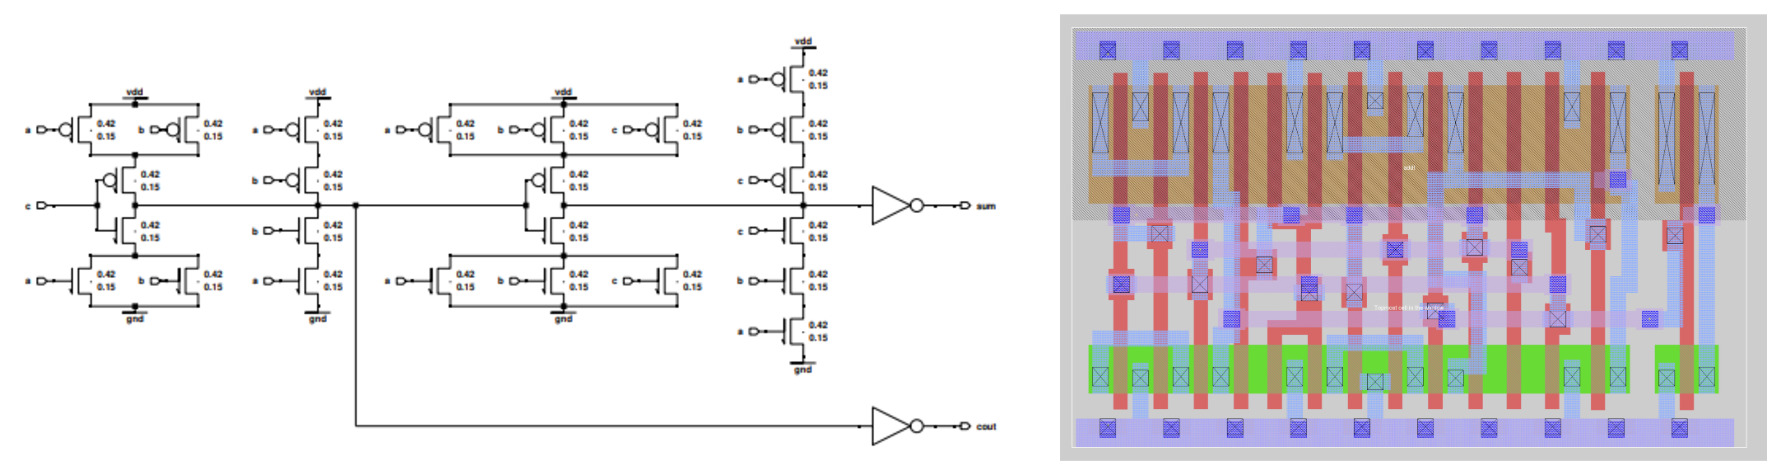
\includegraphics[width=1.0\linewidth]{given1.jpg}
    \caption{Mirror Adder, Transistor Sch. left, Layout right }
    \label{fig:given1}
\end{figure}


Also, a transistor schematic for a D-flip flop, is provided; it utilizes transmission gates in its design, however it lacks any enable based control, which is a design constraint. The schematic, if valid, will need to be designed in layout, and tested further. There is a sample image of the layout for this design, however it still needs to be built from scratch, then modified for the enable functionality. 


\begin{figure}[H]
    \centering
    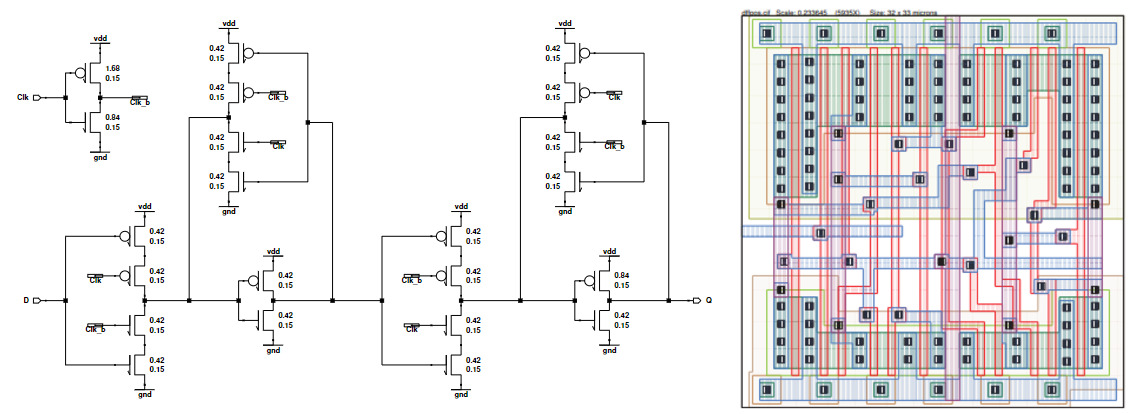
\includegraphics[width=1.0\linewidth]{given2.jpg}
    \caption{DFF, Transistor Sch. left, Layout right }
    \label{fig:given2}
\end{figure}


As for the final required component for the design, the Multiplexer (Mux), has a sample, gate based idea of how it might be built. Therefore, it will be necessary to build the entire Mux, Gate level, Transistor level, stick diagram, and built in layout; as well as testing along the way.

\begin{figure}[H]
    \centering
    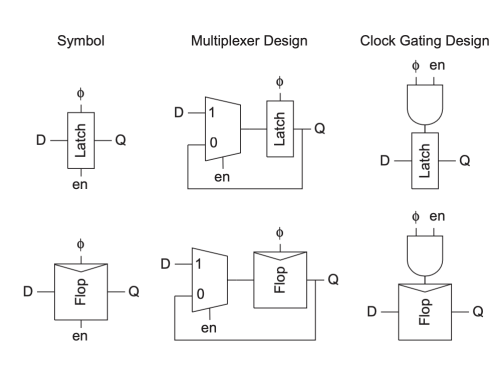
\includegraphics[width=0.7\linewidth]{mux_design.PNG}
    \caption{Multiplexer design options}
    \label{fig:given3}
\end{figure}
 
\subsection{Objectives}

After considering what is given, the strategy will be to understand the larger circuit, and break it done into individual modular components that can be built and tested individually, and then re-integrated back into the larger design, piece by piece. 
\newline
\subsubsection{Mirror Adder}
In this top down approach, it is necessary to build and simulate the circuit before even attempting to do layout or LVS. Since the Adder was given, it will be the first part modeled in Sue, and logically tested with IRSIM to verify it indeed, could do 1-bit binary addition.
\newline
Once the Adder has been verified for logical functionality, a separate schematic is created in Xschem for tested at a later time.
\newline
\subsubsection{D-Flip Flop}

The D Flip-flop also had a low transistor count schematic provided, and it is the next device to be built in tested. A secondary design would be necessary to achieve the clock signals, and a third design would also be necessary to achieve the enable based functionality as ordered in the project outline.
\newline 
As before, the D Flip-Flop will also be modeled in Xschem for additional testing.

\subsubsection{Multiplexer}
When designing the Multiplexer, there are two valid designs: a dual NAND structured device, or a transmission gate approach that will use additional inverters for stability, and output logic. Overall, both perform the exact same functionality, and will be compatible with the rest of the design. However, the Transmission gate approach may offer a lower transistor count, and therefore a simpler design. Unfortunately, the device was first constructed with the NAND approach, and the designed worked without issue, thus it was not replaced. 

%%%%%%%%%%%%%%%%%%%%%%%%%%%%%%%%%%%%%%%%%%%%%%%
\section{Circuit Design}
Below is the overall circuit design
\subsection{Top Level}

\begin{figure}[H]
    \centering
    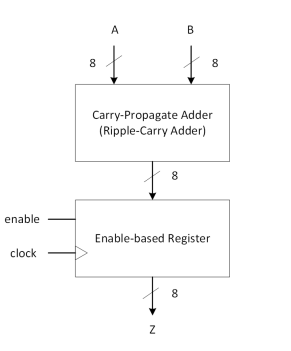
\includegraphics[width=0.5\linewidth]{top_level.PNG}
    \caption{Block Diagram of Top level}
    \label{fig:top_level}
\end{figure}


\subsection{Transistor Level}

\subsubsection{Full Adder}
Here is the Full Adder Layout in Sue.
\begin{figure}[H]
    \centering
    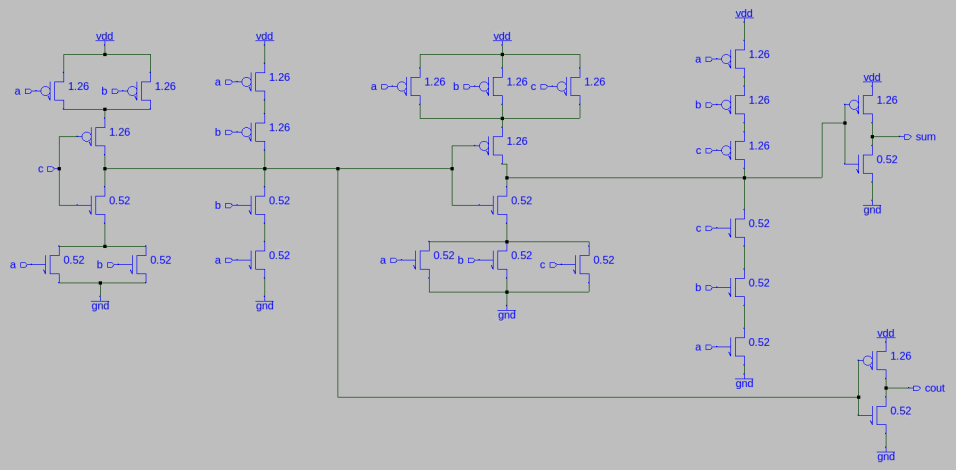
\includegraphics[width=0.8\linewidth]{Adder.PNG}
    \caption{Full Adder in Sue}
    \label{fig:adder_sue}
\end{figure}
Full Adder Testing with IRSIM
\begin{figure}[H]
    \centering
    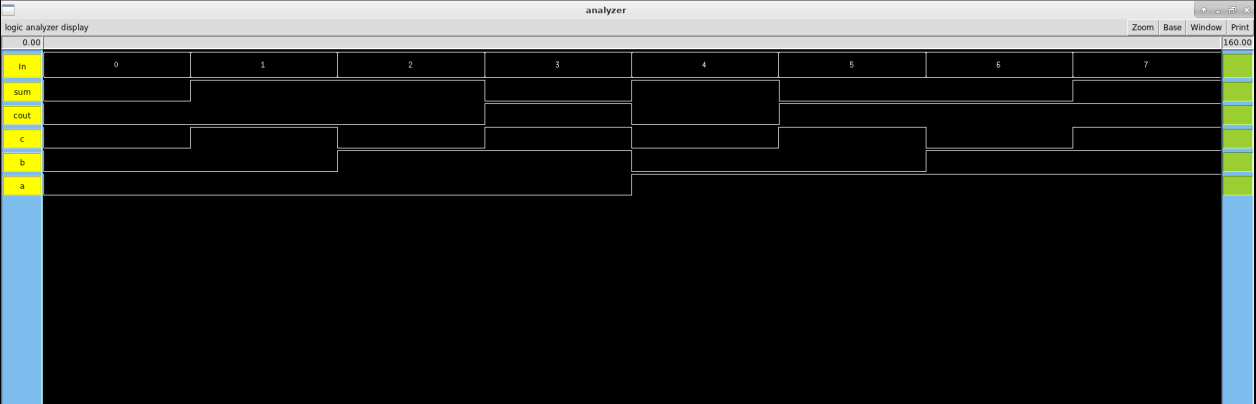
\includegraphics[width=0.8\linewidth]{adder_sim.PNG}
    \caption{Full Adder IRSIM}
    \label{fig:adder_sim}
\end{figure}

\subsubsection{D Flip-Flop}
Here is the D flip flop layout in Sue.

\begin{figure}[H]
    \centering
    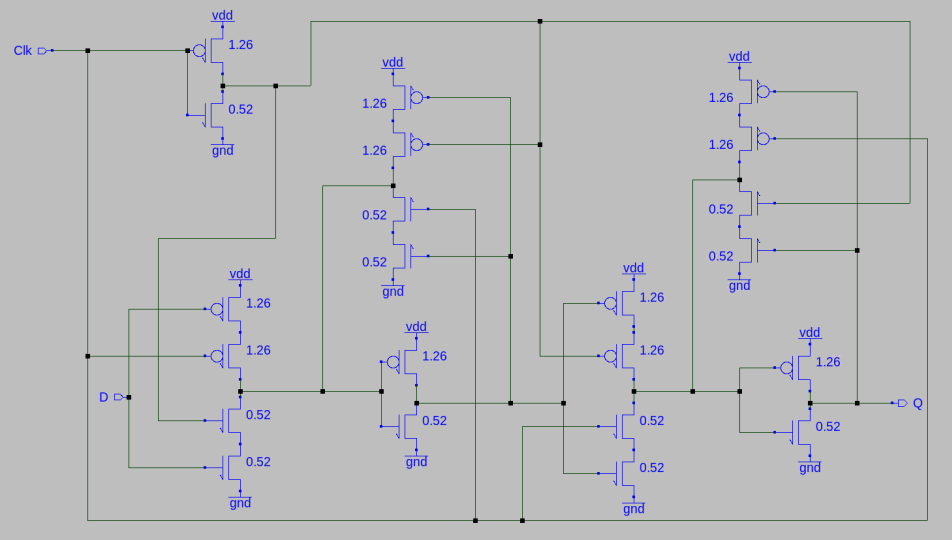
\includegraphics[width=0.8\linewidth]{FF.PNG}
    \caption{D Flip-Flop w/o EN in Sue}
    \label{fig:ff_sue}
\end{figure}

\begin{figure}[H]
    \centering
    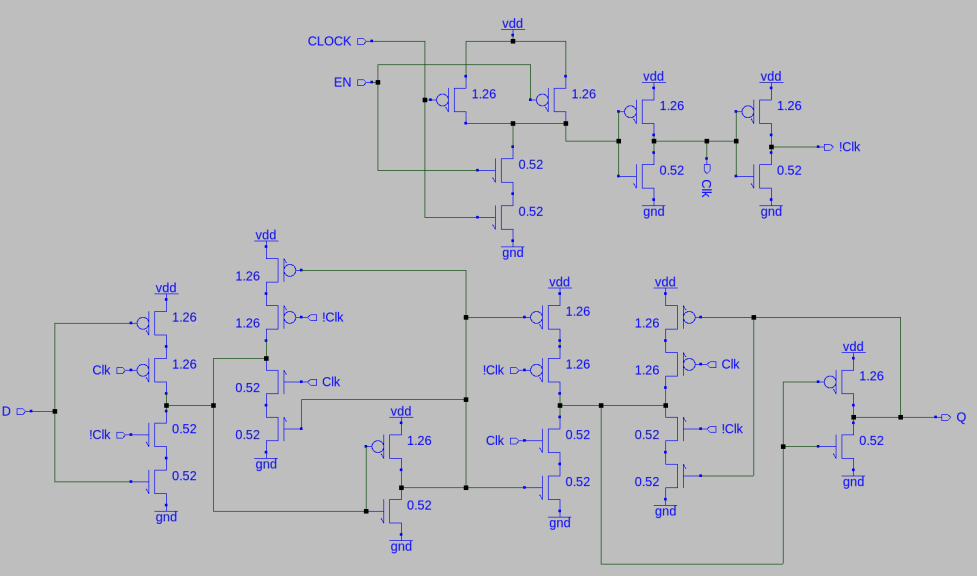
\includegraphics[width=0.8\linewidth]{FF_EN.PNG}
    \caption{D Flip-Flop with EN, in Sue}
    \label{fig:ff_en_sue}
\end{figure}

D flip-flop with EN, in IRSIM

\begin{figure}[H]
    \centering
    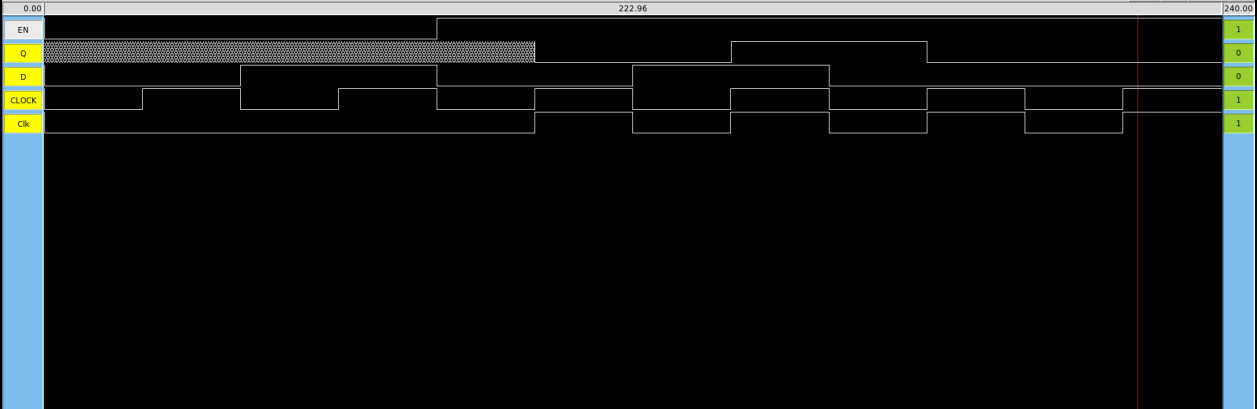
\includegraphics[width=0.8\linewidth]{ff_en_sim.PNG}
    \caption{D Flip-Flop simulation}
    \label{fig:ff_en_sim}
\end{figure}

\subsubsection{Multiplexer}
Here is the Multiplexer layout in Sue.

\begin{figure}[H]
    \centering
    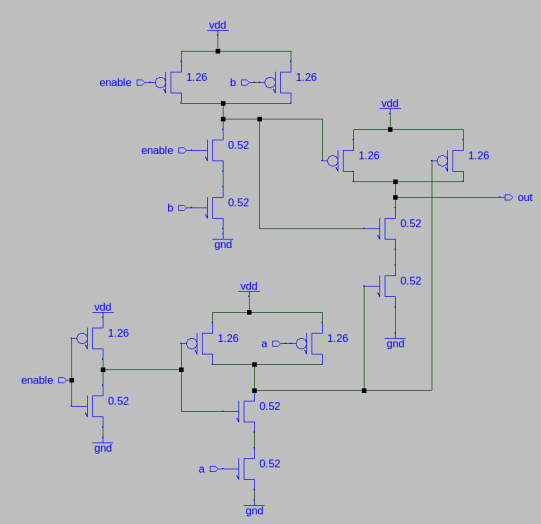
\includegraphics[width=0.8\linewidth]{Mux.PNG}
    \caption{Multiplexer in Sue}
    \label{fig:mux_sue}
\end{figure}

Multiplexer simulation in IRSIM

\begin{figure}[H]
    \centering
    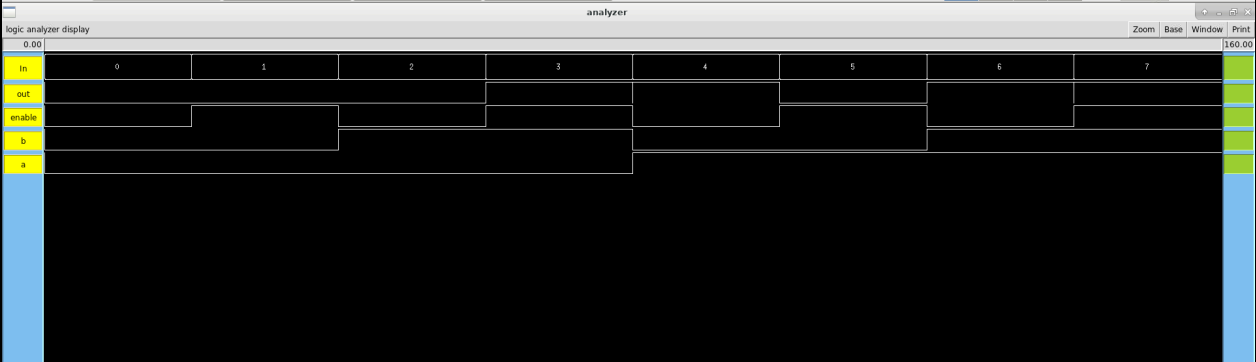
\includegraphics[width=0.8\linewidth]{mux_sim.PNG}
    \caption{Multiplexer simulation in IRSIM}
    \label{fig:mux_sim}
\end{figure}


\subsection{1-Bit Path Assembly}
1-Bit Path Assembly:
\begin{figure}[H]
    \centering
    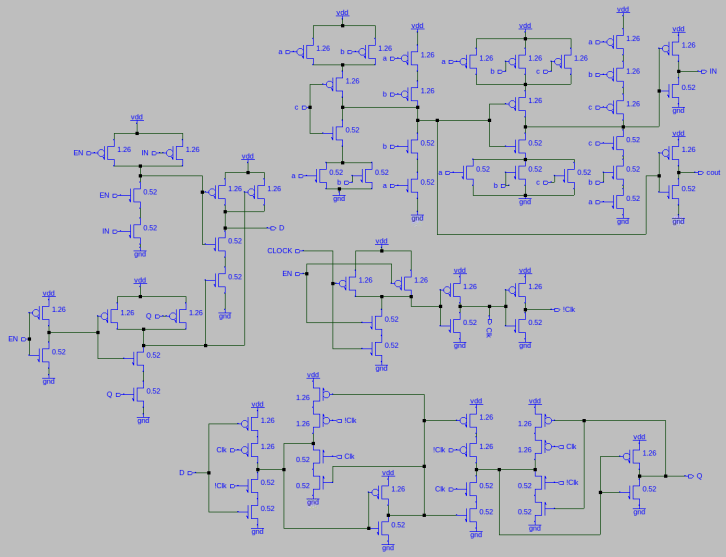
\includegraphics[width=0.8\linewidth]{1Bitpath.PNG}
    \caption{1-bit path}
    \label{fig:1bit_sue}
\end{figure}

1-bit path assembly testing:

\begin{figure}[H]
    \centering
    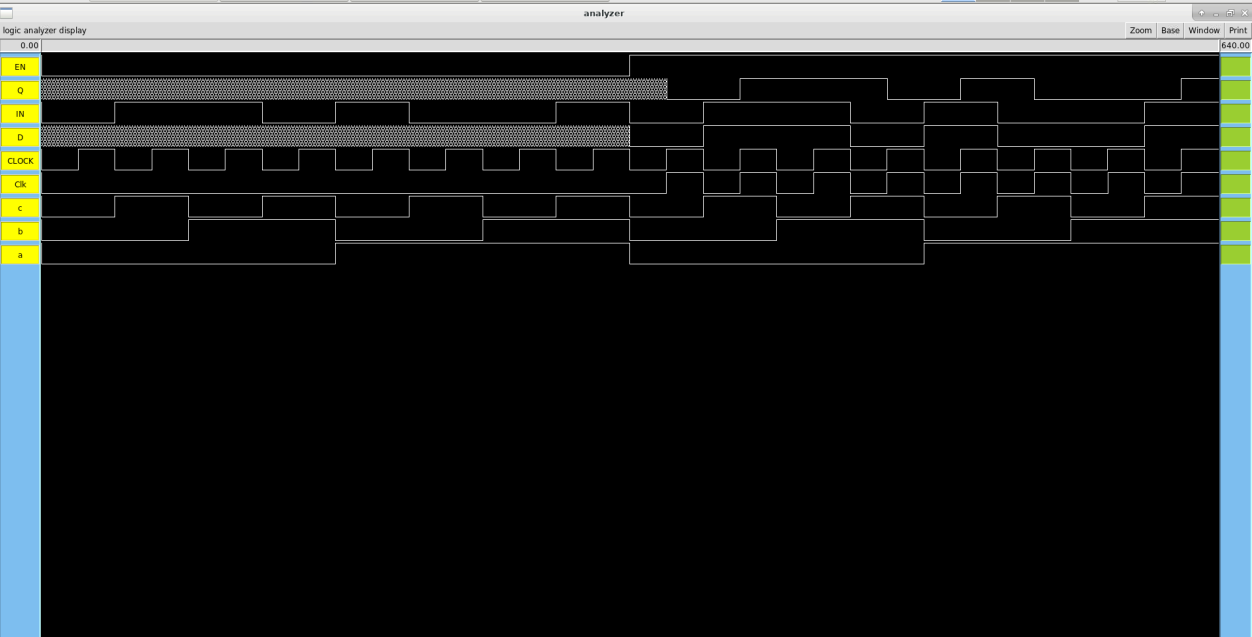
\includegraphics[width=0.8\linewidth]{1bitpath_sim.PNG}
    \caption{1-bit path}
    \label{fig:1bitpath_sim}
\end{figure}

%%%%%%%%%%%%%%%%%%%%%%%%%%%%%%%%%%%%%%%%%%%
\section{Xschem}
\subsection{Adder}
\begin{figure}[H]
    \centering
    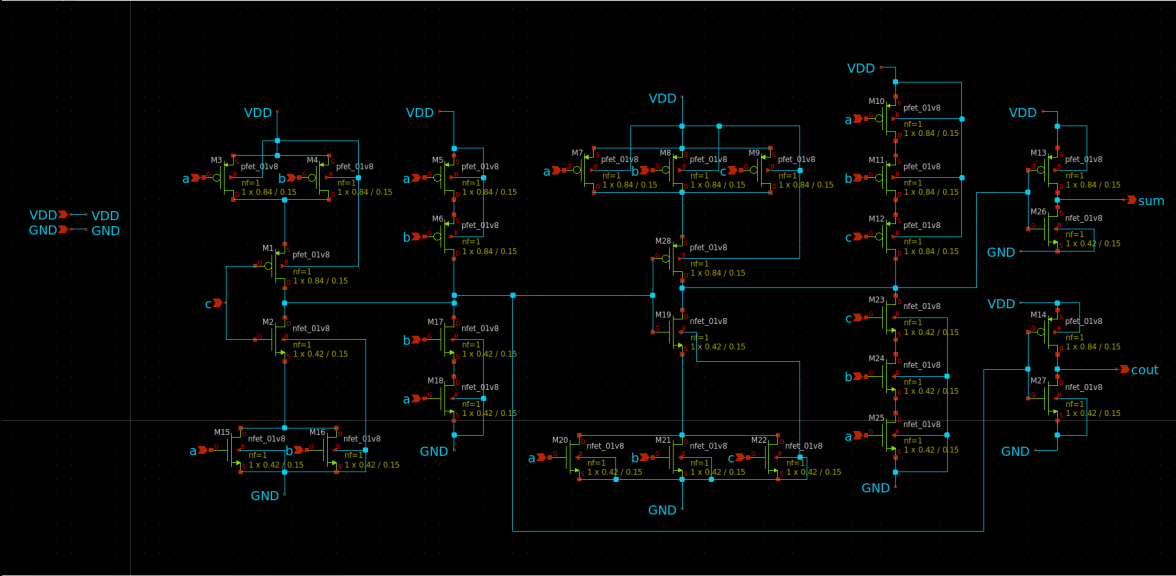
\includegraphics[width=0.8\linewidth]{adder_x.PNG}
    \caption{Adder in Xschem}
    \label{fig:add_x}
\end{figure}

\subsection{D Flip-Flop with Enable}
\begin{figure}[H]
    \centering
    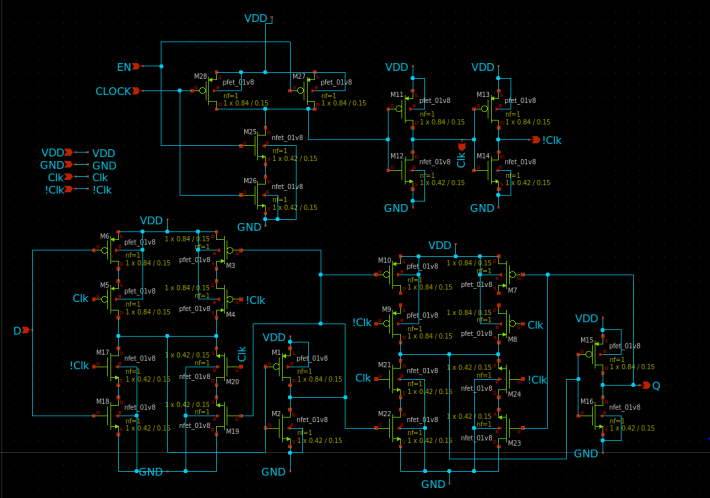
\includegraphics[width=0.8\linewidth]{ff_en_x.PNG}
    \caption{FF in Xschem}
    \label{fig:ff_en_x}
\end{figure}

\subsection{Multiplexer}
\begin{figure}[H]
    \centering
    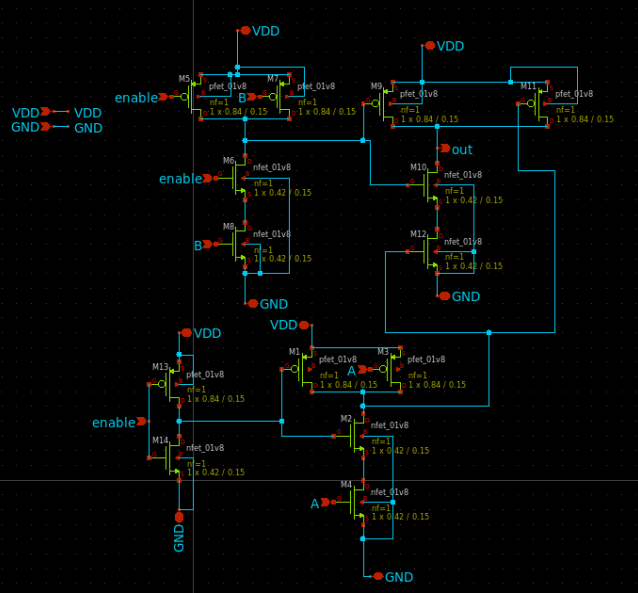
\includegraphics[width=0.8\linewidth]{mux_x.PNG}
    \caption{Multiplexer in Xschem}
    \label{fig:mult_x}
\end{figure}

%%%%%%%%%%%%%%%%%%%%%%%%%%%%%%%%%%%%
\section{Layout}
In order to perform well and minimize layout errors, we can utilize a process of stick diagramming. We will use this to help visualize how a transistor level design can be recreated in layout. Before starting layout, we will walk through the simple stick diagrams for each of the project's components.
\subsection{Stick Diagrams}

\subsubsection{Adder}

\begin{figure}[H]
    \centering
    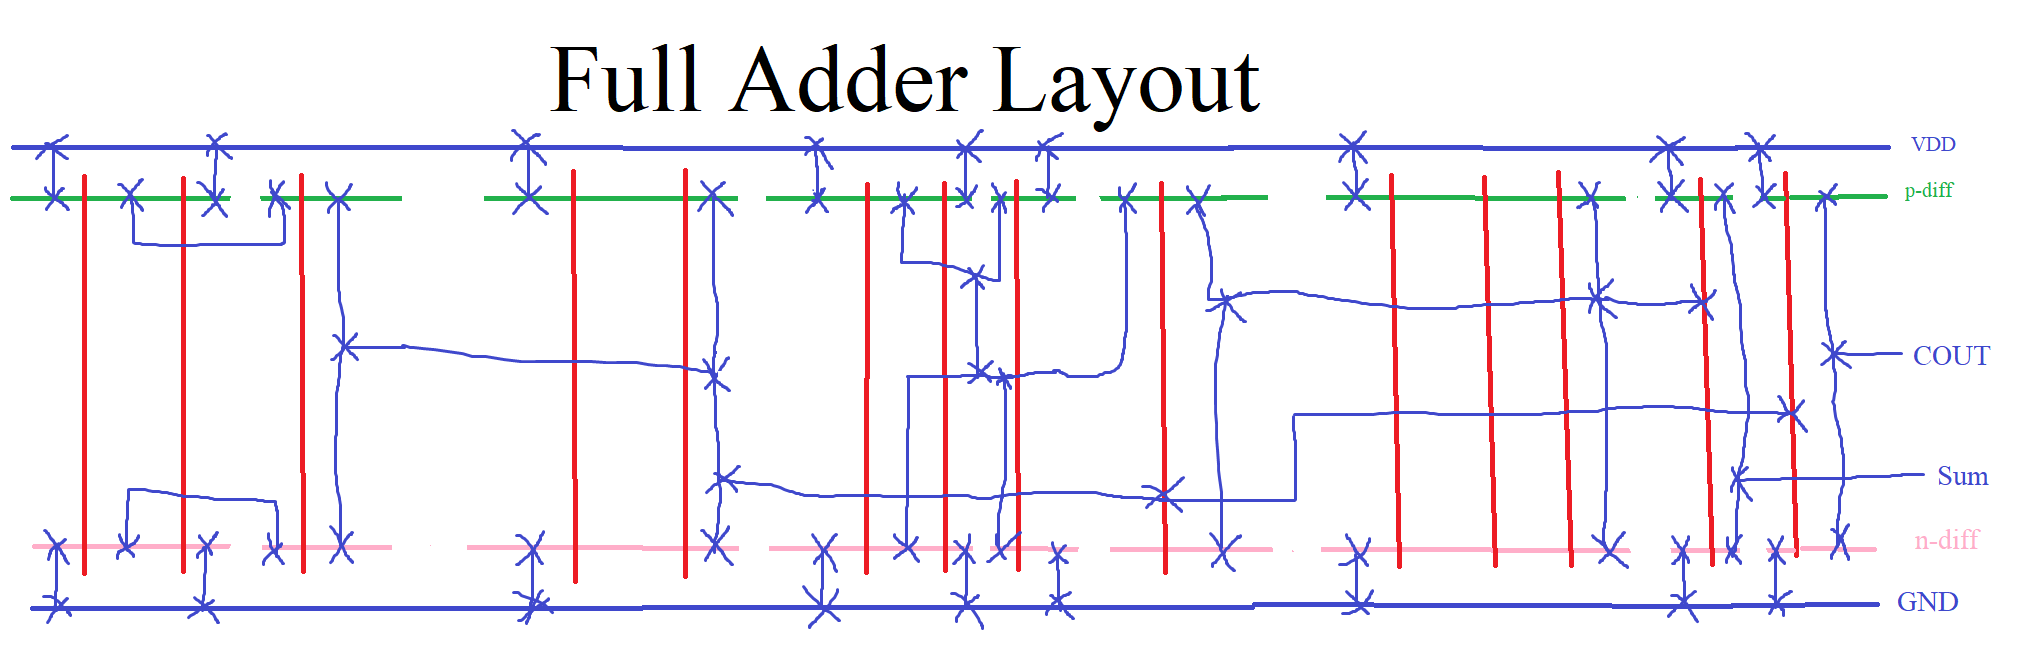
\includegraphics[width=0.8\linewidth]{fulladder_stick.png}
    \caption{Stick Diagram of Adder}
    \label{fig:adder_stick}
\end{figure}

\subsubsection{D-ff}

\begin{figure}[H]
    \centering
    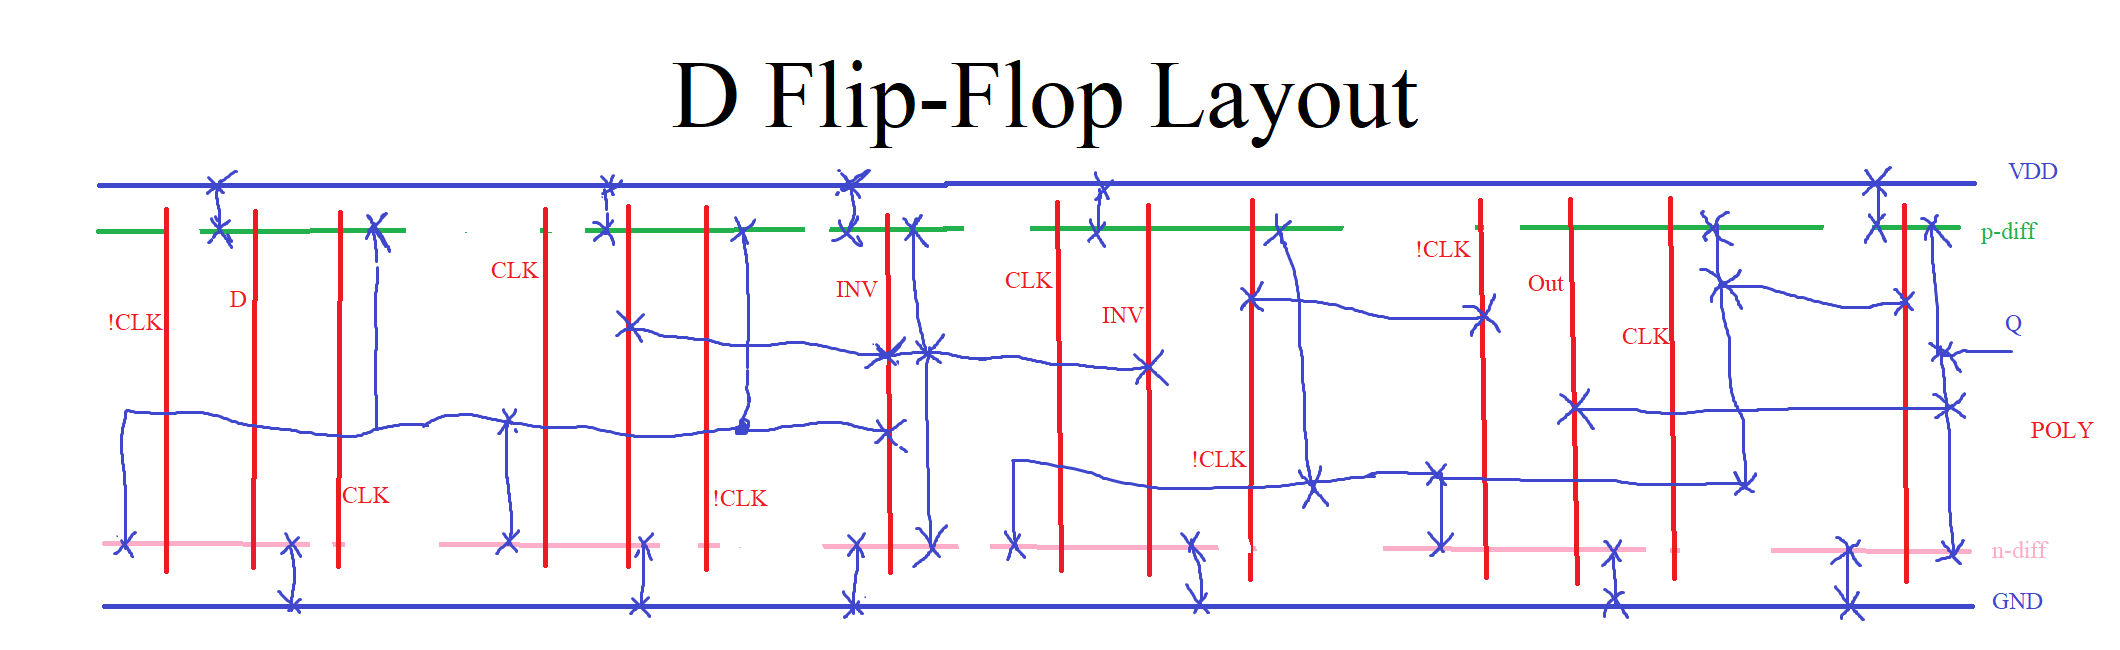
\includegraphics[width=0.85\linewidth]{dff_stick.png}
    \caption{Stick Diagram of DFF}
    \label{fig:dff_stick}
\end{figure}
\begin{figure}[H]
    \centering
    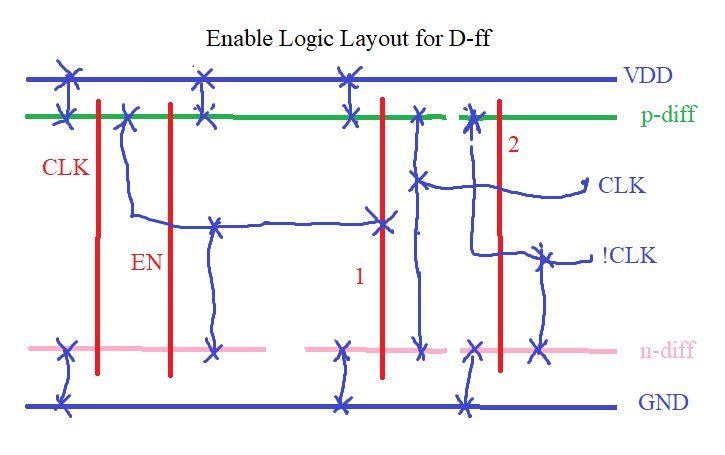
\includegraphics[width=0.6\linewidth]{Enable_stick.png}
    \caption{Stick Diagram of Enable for DFF}
    \label{fig:en_stick}
\end{figure}


\subsubsection{Multiplexer}

\begin{figure}[H]
    \centering
    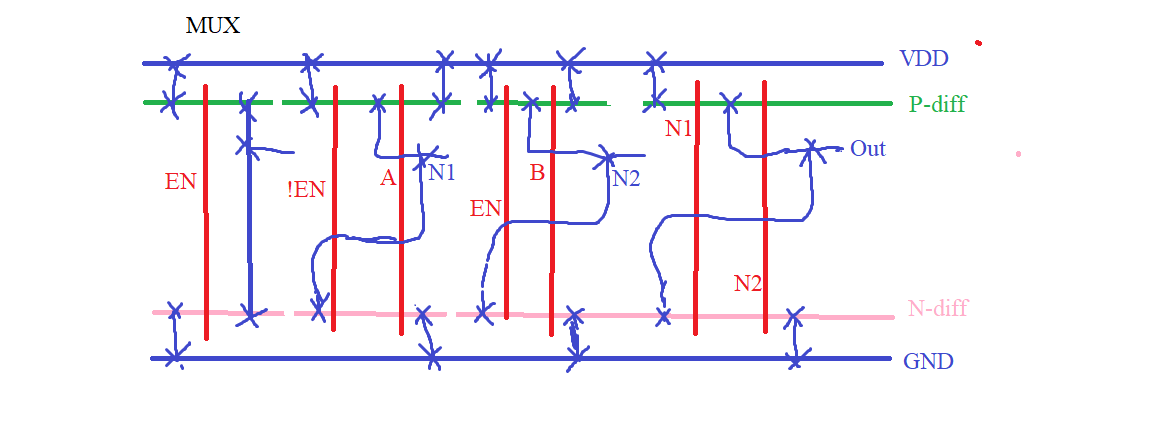
\includegraphics[width=0.8\linewidth]{mux_stick.png}
    \caption{Stick Diagram of Multiplexer}
    \label{fig:mux_stick}
\end{figure}

\subsection{Magic Layouts}

\subsubsection{Adder}

\begin{figure}[H]
    \centering
    \includegraphics[width=0.8\linewidth]{adder_layout.PNG}
    \caption{Layout of Adder}
    \label{fig:add_layout}
\end{figure}

\subsubsection{D-flip flop}
The D-flip flop is expected to be modeled after the stick diagram.
\subsubsection{Multiplexer }
The Multiplexer is expected to be modeled after the stick diagram.


%%%%%%%%%%%%%%%%%%%%%%%%%%%%%%%%%%%%%%%%%%%%%
%\section{Results}
%\subsection{Critical Path and Timing}
%\subsection{Performance}

%%%%%%%%%%%%%%%%%%%%%%%%%%%%%%%%%%%%%%%%%%%%%%%
\section{Files and Documents}
\subsection{Repository}
The project files will be submitted with this document, however more can be found on the project repository:
\newline \newline
\indent https://github.com/mimccom/4303-VLSI-Final-Project
\newline \newline
The project can be cloned with:
\newline \newline
\indent git clone https://github.com/mimccom/4303-VLSI-Final-Project.git

%%%%%%%%%%%%%%%%%%%%%%%%%%%%%%%%%%%%%%%%%%%%%%%
\section{Conclusions}
Utilizing the bit slice technique, this project aimed to forge a streamlined custom data path for an adder and a register. Success was contingent upon generating intricate schematics for logic simulation, ensuring compliance through Spice and LVS with xschem, and culminating in the layout of a bespoke data path in VLSI Magic. This endeavor aimed not only for functionality but also for efficiency, harnessing the power of modular design to optimize performance.
\end{document}